\documentclass[10pt]{article}
\usepackage[utf8]{inputenc}
\usepackage[T1]{fontenc}
\usepackage[polish]{babel}
\usepackage{times}
\usepackage[a4paper, total={6in, 9in}]{geometry}
\usepackage{graphicx}
\usepackage{pythonhighlight}
\usepackage{subfig}
\graphicspath{ {.} }


\title{
\rule{\linewidth}{3pt}
Klasyfikator ruchów czujnika IMU na podstawie rekurencyjnej sieci neuronowej
\rule{\linewidth}{1pt}
}
\author{
  \textbf{Mateusz Woźniak}\\
  \texttt{wozniakmat@student.agh.edu.pl}
  \and
  \textbf{Maciej Pawłowski}\\
  \texttt{maciekp@student.agh.edu.pl}
}
\date{}

\begin{document}

\maketitle

\section{Abstrakt}

Przedmiotem tego artykułu jest omówienie realizacji zadania klasyfikacji ruchów z urządzenia IMU (Inertial Measurement Unit). Czujnik IMU określa przyśpieszenia postępowe i kątowe używając żyroskopu, akcelerometru i magnetometru. 
IMU jest powszechnie stosowane w lotnictwie, robotyce, wirtualnej rzeczywistości i medycynie. W lotnictwie umożliwia precyzyjne sterowanie statkami powietrznymi, a w robotyce wspomaga autonomiczne poruszanie się robotów. Jednym z zastosowań klasyfikatora ruchów może być detekcja przeciągnięcia samolotu. Z kolei w motoryzacji, IMU znajduje użycie w systemach kontroli stabilności pojazdów oraz w zaawansowanych systemach wspomagania kierowcy, które poprawiają bezpieczeństwo. My chcemy zaproponować realizację klasyfikatora 5 z góry ustalonych ruchów używając rekurencyjną sieć neuronowej. 
\\\\Do pomiarów wykorzystaliśmy smartfon Samsung Galaxy S10e 2019 wyposażony w czujnik IMU. Implementację modelu wykonaliśmy we frameworku PyTorch. Trening sieci neuronowej była wykonywany na Apple Macbook M1 16GB.

\section{Zbiór danych}
Dane zostały zebrane z urządzenia Samsung Galaxy S10e 2019. Każdy ruch został zebrany ręcznie a seria danych z czujników była zapisywana do pliku $csv$ o ilości wierszy takiej jak ilość kroków czasowych. Interwał samplowania pomiaru z czujnika ustaliliśmy na $50ms$. To znaczy, że w ciągu każdej sekundy trwania ruchu następowało 20 odczytów.

Ruchy były wykonywane przy włączonej aplikacji mobilnej napisanej w Kotlinie (rys. 1).

\begin{figure}
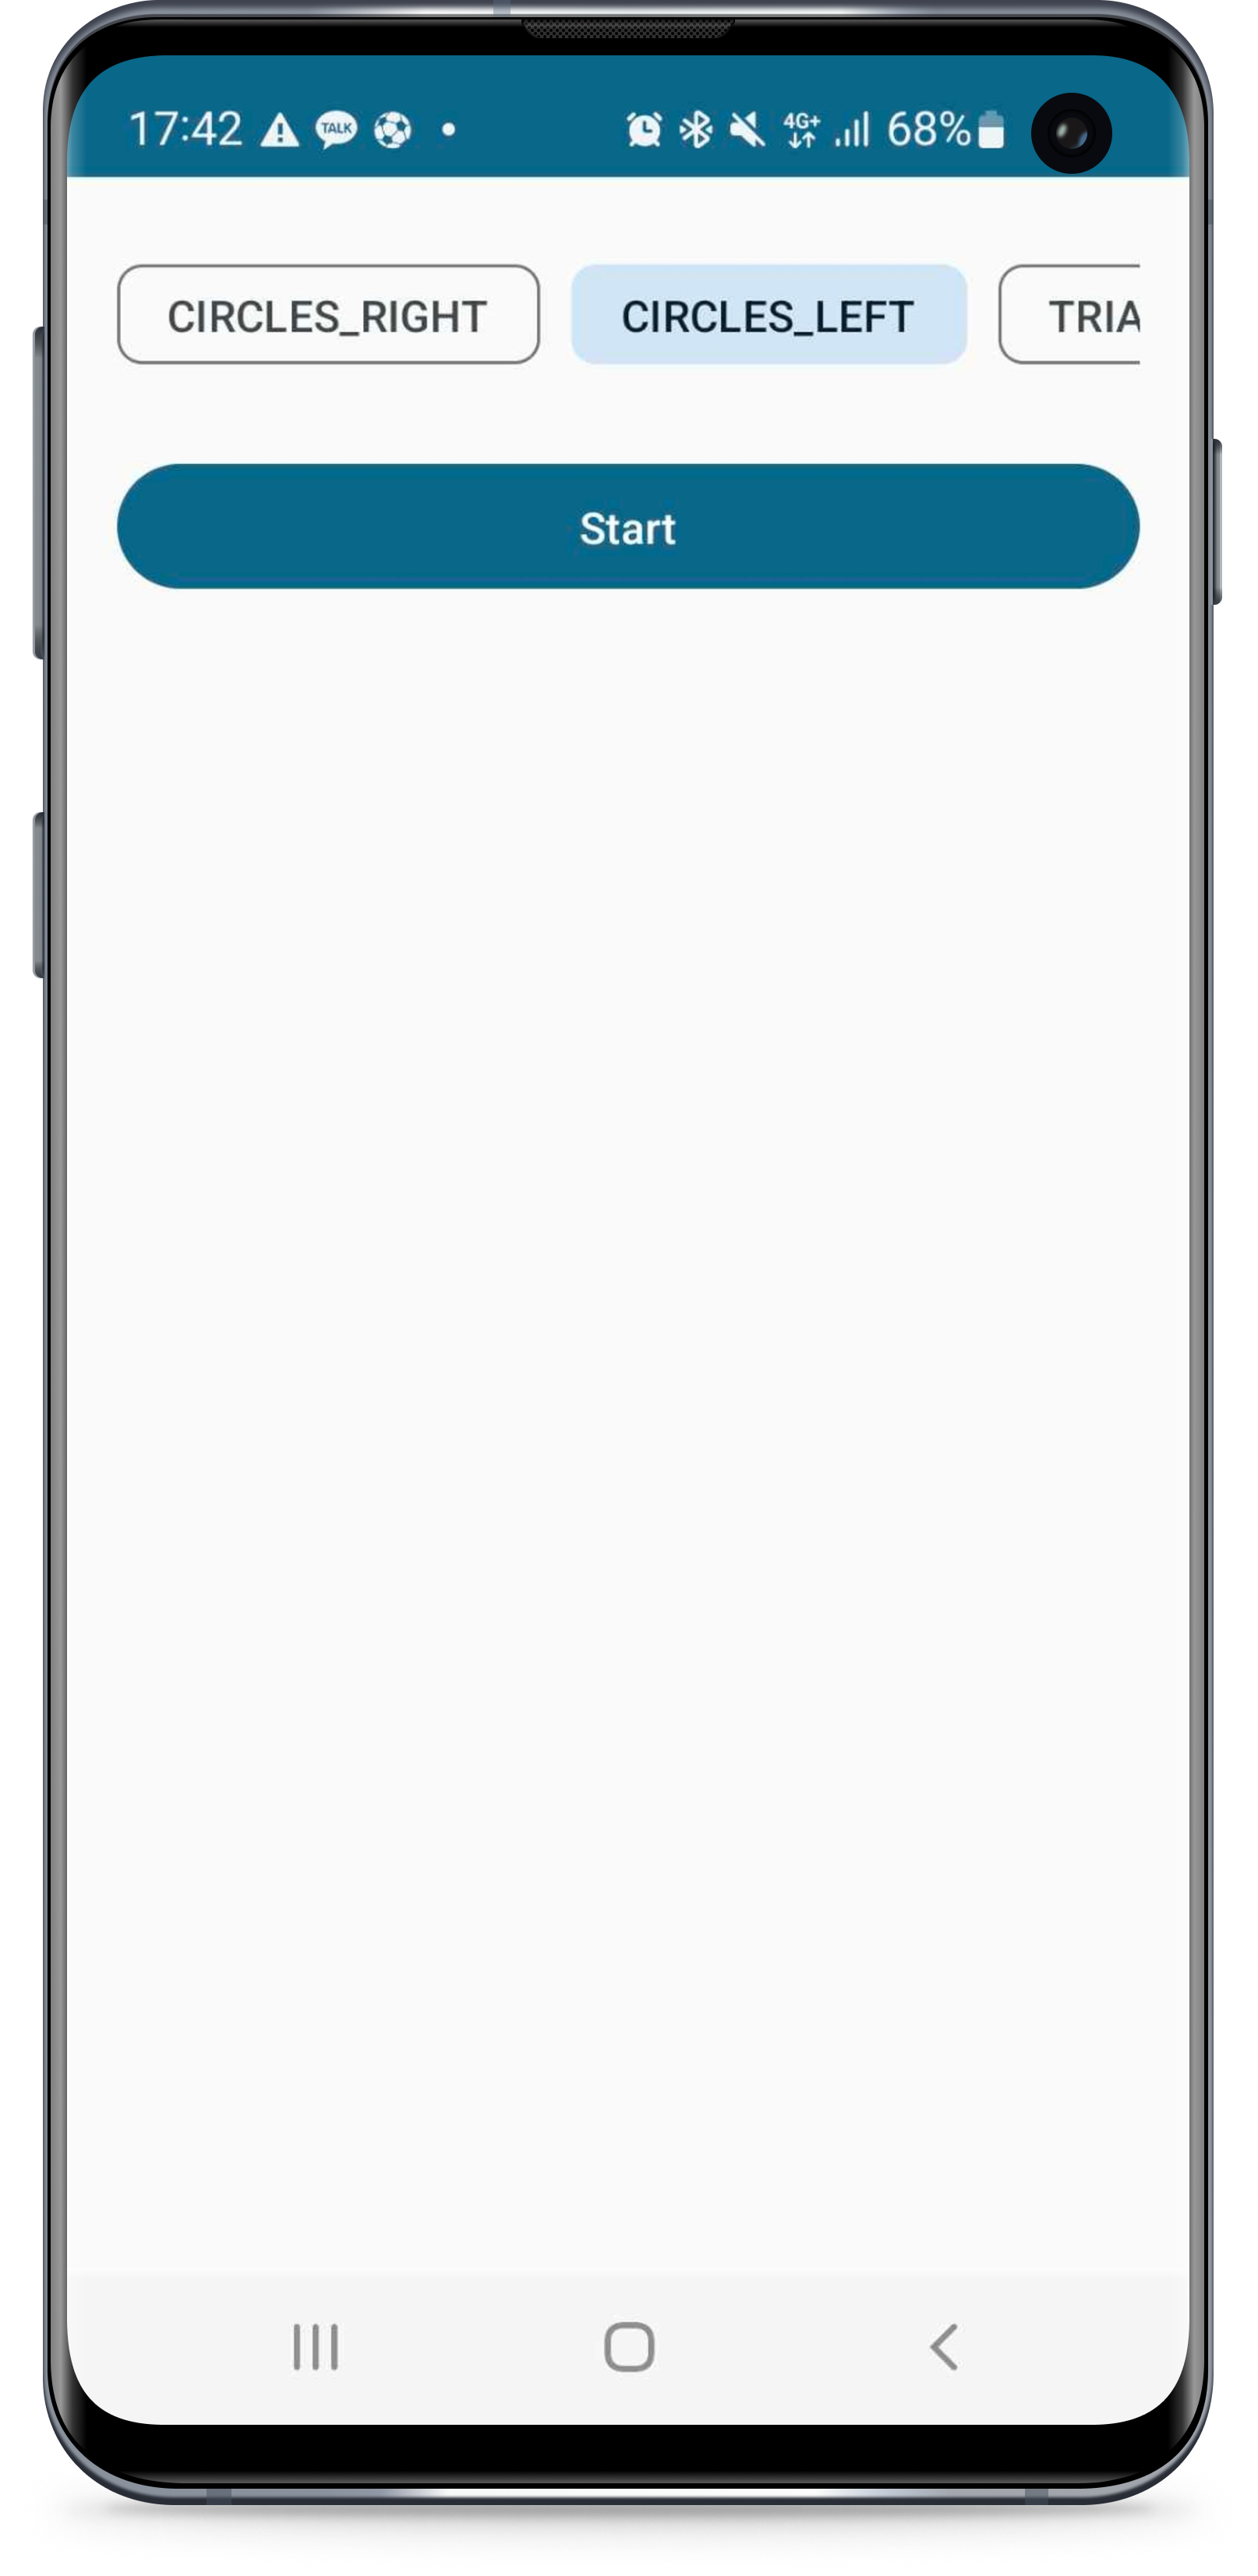
\includegraphics[width=5cm]{s1.png}
\centering
\caption{Aplikacja mobilna do zbierania danych z czujnika IMU}
\end{figure}

Dane były wysyłane na zdalny serwer na którym był uruchomiony mikroserwis HTTP napisany w Go. Mikroserwis zbierał dane i zapisywał je na dysk. Dzięki temu zbieranie danych odbywało się sprawnie, a mikroserwis dawał nam informacje o ilości ruchów dla każdej z klas.

Przykładowy plik $csv$:
\begin{verbatim}  
gyro_x;gyro_y;gyro_z;magnetometer_x;...
-0.062384613;-0.15294538;-0.32650748;-43.62;...
-0.87361366;0.41210496;-0.49510628;-43.5;...
-1.7758616;0.20685424;-1.4266758;-43.92;...
-1.8662697;-0.46876273;-1.4040737;-44.399998;...
-0.7575493;-0.8077929;-1.488984;-44.28;...
0.06895141;-1.5170075;-2.1273382;-46.14;...
\end{verbatim}

Zebraliśmy dane dla następujących klas:

\begin{center}
\begin{tabular}{ |c|c|c| } 
  \hline
  Klasa & Opis ruchu & Ilość sampli \\ 
  \hline
  SQUARE & Ruch imitujący rysowanie kwadratu & 203 \\ 
  \hline
  TRIANGLE & Ruch imitujący rysowanie trójkąta & 179 \\ 
  \hline
  CIRCLES\_LEFT & Rysowanie okręgu przeciwnie z ruchem wskazówek zegara & 193 \\
  \hline
  CIRCLES\_RIGHT & Rysowanie okręgu zgodnie z ruchem wskazówek zegara & 191 \\
  \hline
  FORWARD\_BACK & Ruch "od siebie - do siebie" & 187 \\
  \hline
\end{tabular}
\end{center}

\section{Model}

Ze względu na to, że zadanie klasyfikacji ruchów ma być niezależne od czasu, tzn. że ruch może zawierać dowolną ilość sampli zdecydowaliśmy się użyć rekurencyjnej sieci neuronowej z komórką LSTM.
Long Short-Term Memory (LSTM) to rodzaj architektury sieci neuronowej rekurencyjnej (RNN), zaprojektowanej w celu przezwyciężenia ograniczeń tradycyjnych RNN w przechwytywaniu i uczeniu się długoterminowych zależności w danych sekwencyjnych. LSTMy zostały wprowadzone przez Seppa Hochreitera i Jürgena Schmidhubera w 1997 roku. Chcemy, aby sieć neuronowa nauczyła się zaleności w czasie pomiędzy zmianami w przyśpieszeniach czujnika. W związku z tym w pierwszym podejściu zdecydowaliśmy sprawdzić architekturę składającą się z 32 komórek LSTM oraz dwóch transformacji liniowych $nn.Linear()$ o wielkości 24 i 5. Na ostatniej warstwie została zastosowana funkcja aktywacji $softmax$ by uzyskać dystrybucję prawdopodobieństwa klas (realizuje to $nn.CrossEntropyLoss()$)


Po kilku próbach znaleźlimy hiperparametry modelu, które dają najlepsze zachowanie sieci. LSTM musi mieć 22 komórki, a warstwa gęsta musi mieć 32 neurony. Przeszukiwanie przestrzeni hiperparametrów zostało zrealizowane metodyką gridsearch. Finalny model ma następującą architekturę:

\begin{python}
import torch
import torch.nn as nn

class Net(nn.Module):
  def __init__(self, input_size):
      super(Net, self).__init__()
      self.lstm = nn.LSTM(input_size, 22, batch_first=True)
      self.fc1 = nn.Linear(22, 32)
      self.fc2 = nn.Linear(32, 5)

  def forward(self, x):
      _, (h_n, _) = self.lstm(x)
      x = h_n[-1, :, :]
      x = self.fc1(x)
      x = self.fc2(x)
      return x
\end{python}


\section{Obserwacje}

Model osiąga zbieżność dostarczając przy tym jakościowe predykcje. Zadanie znajdowania zależności między odczytami dalego od siebie nie jest trywialne, aczkolwiek optymalizator jest w stanie znaleźć odpowiedni kierunek by dostosować wagi sieci (rys. 2).
Użyty optymalizator to $Adam$ ze współczynnikiem uczenia $0.001$
 Uzyskana precyzja to ok. 90\% (rys. 3). 

\begin{figure}
  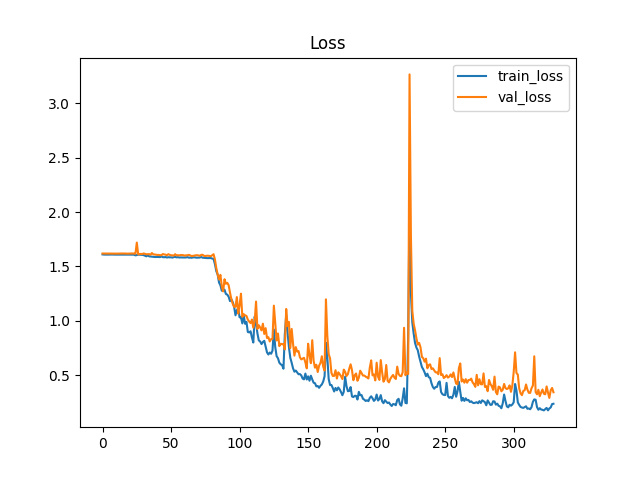
\includegraphics[width=13cm]{loss.png}
  \centering
  \caption{Wykres funkcji straty}
\end{figure}

\begin{figure}
  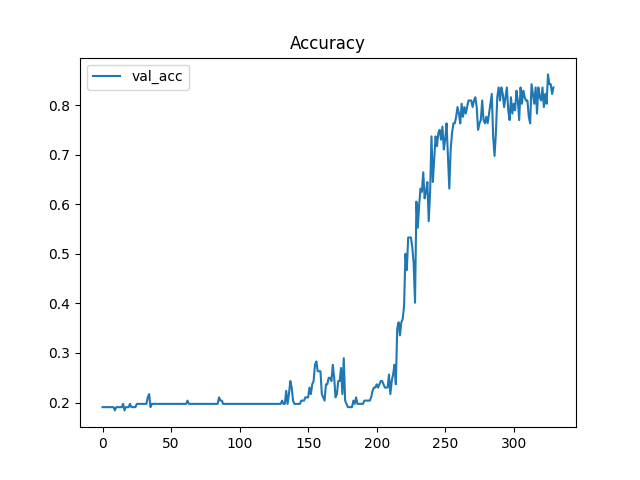
\includegraphics[width=13cm]{acc.png}
  \centering
  \caption{Wykres precyzji na zbiorze walidacyjnym}
\end{figure}

\section{Wnioski}

c

\end{document}